\documentclass[conference]{IEEEtran}
\IEEEoverridecommandlockouts
% The preceding line is only needed to identify funding in the first footnote. If that is unneeded, please comment it out.
\usepackage{cite}
\usepackage{amsmath,amssymb,amsfonts}
\usepackage{algorithm}
\usepackage{algorithmic}
\usepackage{graphicx}
\usepackage{textcomp}
\usepackage{xcolor}
\usepackage{caption}
\usepackage{subcaption}

\graphicspath{{images/}}
\begin{document}

\title{Evolving Bitstrings to Generate Music: A Comparison of Fitness Functions\\}

\author{\IEEEauthorblockN{Akeel Ather Medina}
\IEEEauthorblockA{\textit{Department of Computer Science} \\
\textit{Habib University}\\
Karachi, Pakistan \\
am05427@st.habib.edu.pk}
\and
\IEEEauthorblockN{Abeer Khan}
\IEEEauthorblockA{\textit{Department of Computer Science} \\
\textit{Habib University}\\
Karachi, Pakistan \\
ak05419@st.habib.edu.pk}
\and
\IEEEauthorblockN{Syed Ammar Mahdi}
\IEEEauthorblockA{\textit{Department of Computer Science} \\
\textit{Habib University}\\
Karachi, Pakistan \\
sm03691@st.habib.edu.pk}
}

\maketitle

\begin{abstract}
This research presents an evolutionary algorithm approach for evolving a music composer. The algorithm runs over a corpus of MIDI musical files and compares the end result to well known musical compositions in order to judge similarity. Different fitness functions are implemented, and their results compared to determine the feasibility of different fitness functions for evolving musical compositions. The output is a set of musical notes generated entirely by the algorithm which exhibit vague musical tendencies. Our results demonstrate that musical composition through an evolutionary algorithm is not a trivial problem. Small changes in chromosome representation and fitness functions are vital to ensuring an aesthetic output.
\end{abstract} 

\begin{IEEEkeywords}
Evolutionary algorithm, Musical rater functions, Correlation coefficient, Music generation.
\end{IEEEkeywords}

\section{Introduction}
Generating music, much like creating visual art, has traditionally been viewed as a creative process not suitable for general computers. What makes a musical piece aesthetically pleasing to listen to is a highly subjective process with great variation across time period, cultures, genres, and individual musical preferences themselves.

Despite this subjectivity in the composition process, music nonetheless follows fixed rules that can be viewed as logical relationships between certain frequencies of sound. The mathematical nature of music is not a new concept, but has been around since ancient times; the Pythagorean scale, named after the Greek mathematician, is a classic example of how tempered tuning between musical pitches can produce a scale that is based on mathematical ratios between individual frequencies of sounds, or \textit{pitches}. Indeed, Western music theory as a whole is based on not only the relationships between individual musical notes, but the complex interplay of three major musical elements: harmony, rhythm, and melody.

So while there is great room for individual subjectivity in the music composition process, the existence of fixed rules that define the relationships between musical sounds is what has paved the way for evolutionary computing approaches to music generation. With these known music theory concepts, one can therefore drastically restrict the vast solution space of generating subjective musical pieces to a much narrower one bounded within a fixed set of rules. In this manner, music composition also becomes a quasi-logical system of sorts that we can thus manipulate with the help of evolutionary algorithms.

In our paper, we implement a well-known process of generating musical pieces using the evolutionary algorithm approach highlighted by Sulyok, McPherson, and Harte\cite{b1}. Specifically, we implement a evolutionary algorithm to model a human composer, the output of which is a byte array corresponding to a musical piece. We also address the limitations cited by the authors and further their work by using more novel fitness tests directly inspired by music theory, namely that of the approach of utilizing musical raters,\cite{b2} and the Normalized Compression Distance\cite{b4}.

The rest of our paper is structured as follows: section II details the technical background of evolutionary algorithms and relevant music theory before offering a brief literature review of evolutionary algorithms in generating music. Section III deals with the problem description, and section IV addresses our specific implementation of the algorithm including the required fitness functions. Finally, the results obtained are presented and discussed further in section V as well as possible directions for future work.

\section{Technical Background}
\subsection{Evolutionary Algorithm}

At its crux, the music composition process can be reduced to an optimization problem, where one seeks to optimize the similarity between a generated musical composition piece and existing musical compositions from the corpus.

The evolutionary algorithm is a computing algorithm inspired directly from the evolution process in nature. It is a meta-heuristic optimization algorithm, meaning that it provides a sufficiently good solution to the problem despite not guaranteeing a globally optimal solution.\cite{b3}. This algorithm is particularly well-suited for musical composition as the solution space is quite large to fully explore, thus a meta-heuristic approach yields a better solution.

A procedural description of the evolutionary algorithm is outlined in \textbf{Algorithm 1}.

\begin{algorithm}
\caption{Evolutionary Algorithm Procedure}
\begin{algorithmic}[1]
\STATE Initialize a random population of individuals.
\STATE Evaluate the fitness of each individual in the population using a fitness function.
\REPEAT
\STATE Select the individuals from the population using a parent selection scheme.
\STATE Use crossover and mutation operations to generate new individuals.
\STATE Evaluate the fitness of the new individuals.
\STATE Replace the least fit individuals of the population with the best new individuals.
\UNTIL Stopping condition is met.
\end{algorithmic}
\end{algorithm}

\subsection{Musical Background}

Music theory details a set of fixed rules that describe the logical relationships between individual musical notes and musical elements of the piece as a whole.

Here are some musical terms that will help better understand the music theory terms used in this research:

\begin{enumerate}
    \item \textbf{Note:} A musical note is a pure frequency of sound, as opposed to noise, which can be a combination of different sounds.
    \item \textbf{Pitch:} The frequency of musical notes in $Hz$. Often characterized into low versus high pitches.
    \item \textbf{Scale:} A set of notes defined in mathematical relation to one another, through the ratios of their relative pitches. 
    \item \textbf{Melody:} A subset of notes from a parent scale that are aesthetically pleasing to listen to when played in sequence.
    \item \textbf{Rhythm:} A periodic movement across time that the musical piece is synchronized with. Rhythms are further divided into \textit{beats}, the atomic unit of a rhythm, and \textit{measures}, a uniform division of time that repeats a combination of beats.
    \item \textbf{Inter-onset-Interval (IOI):} The time elapsed between the start of the previous note and the start of the current note.
    \item \textbf{Duration:} The length of time a note plays for.
\end{enumerate}

A track is made up of a set of notes. Each note in a track has a set of distinct properties such as velocity, pitch, duration, start, end, etc. For the purpose of our research, we will primarily focus on three note properties; pitch, IOI, duration. 

\subsection{Previous Work}

The use of evolutionary algorithms for generating music is hardly a new research area. Early research in this area began since the 1990s, with Gibson \& Byrne\cite{1991} presenting some of the earliest implementations. These early implementations, however, suffered from a lack of objectivity when it came to the fitness functions.

It was not until the inclusion of musical elements such as melody\cite{b4}, harmony\cite{harmony}, and other performance elements that the solution space of music composition using evolutionary algorithms was greatly reduced. Another approach to reduce the vast solution space of generated music has been to shift the focus from finding better fitness functions to setting up the initial population with non-randomized human-generated musical compositions and evolving the compositions from there\cite{nonrandom}.

A major breakthrough was achieved by first utilizing a virtual composition to focus on the music composition process itself as opposed to generating musical pieces\cite{composer}. As mentioned, this approach was furthered by Sulyok, McPherson, and Harte \cite{b1}. Our work furthers their approach by addressing the limitations of their research to incorporate and compare different fitness functions that more directly address musical elements such as harmony. However, rather than evolve the music through a virtual machine composer, we restrict the domain to generating music via bitstring manipulation. The fitness evaluation approach of using musical raters and subraters\cite{b2}, which aggregate different musical qualities, has also been fruitful in introducing more objective fitness functions that can better measure the musical qualities of a given piece.

\section{Problem Description}
How can evolutionary algorithms compose and render musical pieces that are musically similar to real music? Although the musical composition seems as an entirely subjective endeavor first glance, the existence of fixed logical rules between musical elements according to music theory allows one to shift the problem from a subjective to an objective one.

Our task therefore becomes one of encoding a fixed set of rules and relations into a parseable format that our evolutionary algorithm can help evolve into combinations. Bitstrings are especially well suited to this task; using a bitstring, one can encode anything ranging from chess moves, video game fighting combinations, or in our case, a musical piece in a simple machine-friendly binary format. The input to the evolutionary algorithm is a bitstring that is encoded with musical note information according to a fixed set of musical rules, and the output is also a bitstring (byte array) which is thus decoded with the same rules to produce a musical piece.

Additionally, given a corpus of real music, a composition program must be able to output musical pieces that are similar to it. To do this, the algorithm needs to be able to define similarity in a meaningful way to evaluate the generated results. There are several ways in which one can define the notion of similarity; one approach is to consider statistical similarity between the corpus and the generated output, whereas another is to  represents the universal distance between two musical scores. This notion of similarity therefore corresponds to our fitness values in our evolutionary algorithm.

\subsection{MIDI Files}
For this implementation, fifteen keyboard tracks from Bach's Inventions and Sinfonias - tracks 772 to 786, were used as the corpus of real music to determine and assess statistical similarities. "This corpus was chosen because it contains relatively short pieces of similar lengths (around 90 s); and also because of its stylistic and structural homogeneity, which we hoped would help narrow the solution space to a certain extent. The files in the corpus have been generated from a score rather then recorded by a human player. As a result they contain no elements of musical expression such as micro-timing variation or changes in dynamics and tempo. All notes have velocity 127, therefore our current system does not use velocity as a note property." \cite{b1}
\section{Implementation}


\subsection{Chromosome}
Each individual, or chromosome, in this implementation is a bitstring (i.e. sequence of $1s$ and $0s$) of length 192. Each chromosome in the population is a binary representation of a musical track, by separating the bitstring into three 64-bit chunks, with each chunk representing a musical property; pitch, IOI and, duration. The pitch, IOI, duration values are randomly initialized during the initial population generation phase.


\subsection{Fitness Functions}
Using three different fitness functions, the fitness of a chromosome is evaluated to judge its similarity against a corpus of real music. A high fitness value indicates that the chromosome is similar to a real musical track.

\subsubsection{Normal Distribution and Descriptor Correlator Tests}
In this, two tests are performed: Normal Distribution, and Descriptor Correlator Tests. The normal distribution test is used for evaluating the total duration and number of notes in a track. The descriptor correlator tests evaluate similarity by assessing the three note properties of a track; pitch, IOI, and duration. The resultant fitness value will depict the statistical similarity of an individual with the corpus of music. \cite{b1}

For the normal distribution test, the mean and standard deviation values are calculated for all lengths and number of notes in the corpus. The result gives 2 values from which a normal distribution can be simulated. Passing the length and number of notes for an individual through this normal distribution gives us a fitness value between 0 and 1 after normalization. The mean of these values is the result of the normal distribution test.

For the descriptor correlator tests, four transform methods are applied to each of the three note properties outlined above to generate twelve statistics to compare with. Firstly, the twelve statistics are calculated for the corpus. Secondly, the twelve statistics are generated for every chromosome in the population. We can compare each statistic between our individual and corpus by the use of the Pearson Correlation Coefficient. This will return a scalar value between 0 and 1. Every track in the corpus will have 12 correlation coefficients generated, and calculating the overall mean will give the output of the descriptor correlator tests.

The four transform methods applied in this implementation are:
\begin{enumerate}
    \item Histogram- for evaluation of the distribution of a particular note property.
    \item Histogram of the Differential- for the evaluation of the rate of change between consecutive notes.
    \item Fourier Transform- for the evaluation of rhythm and patterns.
\item Fourier Transform of the Differential- for the evaluation of the repeating patterns in the rate of change between consecutive values.
\end{enumerate}

The mean of the 2 test results gives the final fitness value \cite{b1}. To summarize, a higher fitness function may indicate a higher similarity in:
\begin{enumerate}
    \item Length of track
    \item Number of notes in track
    \item Specific notes used
    \item Specific contours note-by-note 
    \item Specific patterns and rhythms
    \item Specific repeating contour patterns
\end{enumerate}


\subsubsection{Normalized Compression Distance}
The NCD, simply put, measures similarity between 2 objects. In our case, the object is a bitstring. We compute the scalar value for similarity between each individual in the population against the members of our corpus. This value can directly be returned as our fitness value. The formula for NCD is as follows:

\begin{center}
NCD(x,y) = ${\frac {\max\{C(xy)\-C(x),C(yx)\-C(y)\}}{\max\{C(x),C(y)\}}}$
\end{center}

A NCD value near 0 represents a higher level of similarity between x and y, while a NCD value near 1 represents a lower level of similarity between x and y. Since our objective is to model a human composer, we want to increase similarity, and thus we minimize the NCD.

\subsubsection{Sub-raters}
To generate an appealing musical score, we can apply a series of sub-raters that each rate our music piece and return a value between 0 and 1. These ratings will give an objective measure of how aesthetically pleasing each musical piece is. Taking the average of each sub-rater will yield the fitness value. The following sub-raters were included in the fitness function: \cite{b2}
\begin{enumerate}
    \item Neighboring Pitch Range
    \item Direction of Melody
    \item Direction Stability of Melody
    \item Pitch Range in Melody
    \item Continuous Silence
    \item Unique Pitch Notes
    \item Equal Consecutive Notes
    \item Unique Rhythm Values
\end{enumerate}
Although this measure of fitness is best used in conjunction with first 2 fitness functions, we have included results separately for the visual comparison.

\subsection{Crossover}

The crossover operator implemented was 2-point crossover. The 2-point crossover allows for a greater preservation of parent genetic material between the two parent chromosomes as compared to the single point crossover.

In 2-point crossover, two crossover points are randomly selected from the parent chromosomes and swapped to produce children with greater genetic variation.

\subsection{Mutation}

The mutation operator implemented was Reverse Sequence Mutation (RSM). RSM was chosen due to its proven superiority over other mutators in solving a known optimization problem: the Traveling Salesman Problem (TSP) \cite{RSM}.

This operation takes a bitstring sequence denoted $S$ and restricts it between two random integers $i$ and $j$, where $i < j$. The input bitstrings are:
\begin{align*}
x_{1} = [x_{(1,1)}, x_{(1,2)}, ..., x_{(1, n)}] \\
x_{2} = [x_{(2,1)}, x_{(2,2)}, ..., x_{(2, n)}]
\end{align*}

which produce the output:
\begin{align*}
y_{1} = [y_{(1,1)}, y_{(1,2)}, ..., y_{(1, n)}] \\
y_{2} = [y_{(2,1)}, y_{(2,2)}, ..., y_{(2, n)}]
\end{align*}
The RSM mutation operator is thus implemented in \textbf{Algorithm 2}.

\begin{algorithm}
\caption{RSM Mutation Operator}
\begin{algorithmic}
\REQUIRE: $i, j \in n$ 
\ENSURE: $1 \leq i \leq j \leq n$
\WHILE{$i < j$}
\STATE $x_{i} = x_{i + 1}$
\STATE $x_{j} = x_{j - 1}$
\ENDWHILE
\end{algorithmic}
\end{algorithm}

\subsection{Selection Schemes}

\subsubsection{Parent Selection - Binary Tournament}

Parents were chosen through binary tournament, the simplest tournament selection scheme. Binary selection with a large tournament size ensures a good selection pressure, thereby guaranteeing that chromosomes with poor fitness do not get selected for crossover.

\subsubsection{Survivor Selection - Truncation}
Using truncation selection, the chromosomes with the worst fitness values are dropped out, and are not carried forward into the next generation. The selection scheme is carried out by sorting the population according to their fitness values.

\section{Experiments}
The experiments were run with an initial randomly generated population of 60 chromosomes. The number of offsprings that were generated using the crossover operator was set to 10. The mutation rate was set 0.2. The number of generations was set to 100. \\
\\
Three types of experiments were run, each implementing a different fitness function, using the same parameters outlined above. 

\section{Results}
\begin{figure}[htbp]
\centerline{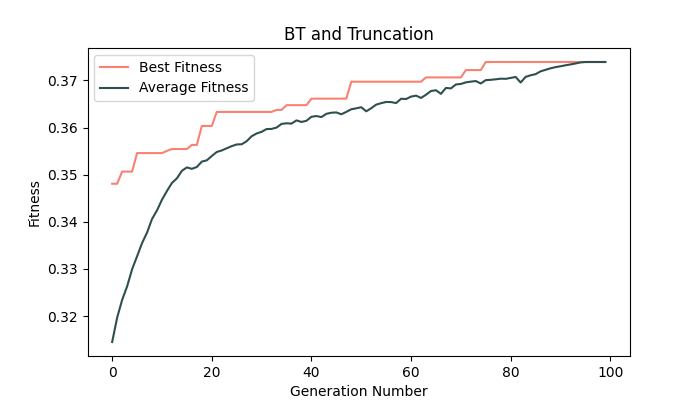
\includegraphics[scale = 0.5]{fitness1-100.png}}
\caption{Normal Distribution and Descriptor Correlator Tests}
\label{fig}
\end{figure}

\begin{figure}[htbp]
\centerline{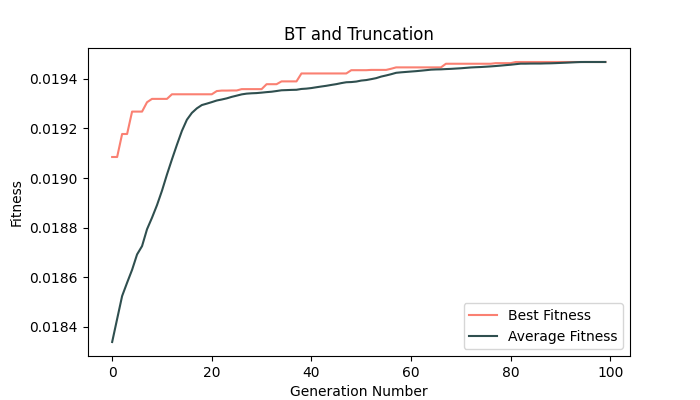
\includegraphics[scale = 0.5]{fitness2-100.png}}
\caption{Normalized Compression Distance}
\label{fig}
\end{figure}

\begin{figure}[htbp]
\centerline{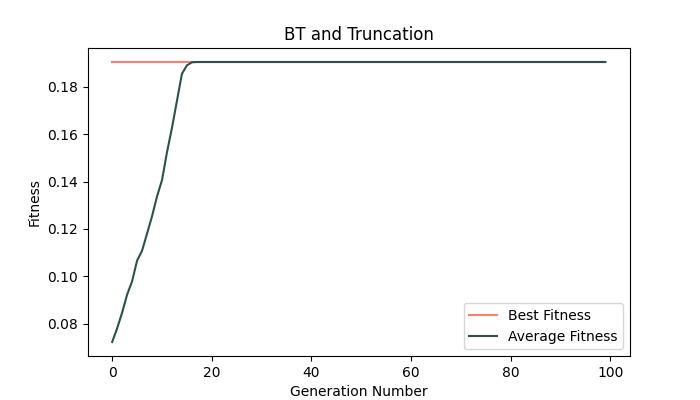
\includegraphics[scale = 0.5]{fitness3-100.png}}
\caption{Sub-raters}
\label{fig}
\end{figure}

Early convergence is reported in all the figures generated. There is a steep increase in fitness value initially, and then the fitness value becomes constant, indicating an early convergence. Increasing the population size and mutation rate to generate increased population diversity provides almost no benefit to the results. 
\\
Due to the early convergence, there isn't enough optimization occurring for the bitstrings to evolve into tracks that appear and musically sound similar to the corpus of real music, but some improvements are observed sonically and visually. Through the analysis of the piano roll observations of the results, it can observed that some changes have occurred when comparing the initial best-so-far chromosome of the first generation and the final best-so-far chromosome of the last generation. When comparing Fig. 7, and Fig. 8, it can be seen in Fig. 8 that the first 30 seconds of the piano roll show a slightly different arrangement of notes than the ones that can be observed in Fig. 7.  Although, an early convergence occurs, this indicates that the normal distribution and descriptor correlator tests are able to assess and optimize the musicality of the music tracks. Observing the complete piano rolls of the tracks shows that there is a disarray of notes as the notes are not arranged in such a way as to construct a pattern that can be observed in Fig. 5. The remaining two fitness functions do appear to have affected the arrangement of the notes of the results when observing Fig. 12, Fig. 13, Fig. 16, and Fig. 17.

Sonically, there are some musical traits that do appear in the final results, such as repetition. Using the normal distribution, and descriptor correlator tests, the results were found "to have motifs of a few notes repeated multiple times, and some show variation on the repeated theme. The system successfully finds small motifs consisting of a few notes which, when repeated many times, allow the result to approach the statistics of the corpus. However, these results are not particularly musical." \cite{b1} Other musical properties such as harmony, melody, and rhythm are absent, primarily due to the fitness functions and the construction of the bitstring to concentrate only on pitch, IOI, and duration. Considering properties like beat time as a note property in the fitness function construction would help bring about more musical traits. 

\section{Conclusion}
This paper aimed to explore the implementation of evolutionary algorithm onto the problem of musical evolution, comparing fitness functions. A musical score in the form of a bitstring was evolved to test for statistical similarity as well as a universal distance from a corpus of music by a single composer, in hopes to mimic specific tendencies and musical properties of this composer. The algorithm was run multiple times and results showed that the evolutionary algorithm
approach was somewhat effective in finding an optimal solution for the
problem. Our results proved the need of logically sound fitness functions in order to generate aesthetically pleasing music. Evolutionary algorithms are ideal for this problem and gave promising results for testing against statistical similarity. Further optimizations can be worked on in the future to improve our results.

\section{Future Work}
There are several promising areas of improvement that can be determined from this paper. \\
This paper tackles this problem using several fitness functions, and only one problem representation. Using different problem representations, such as variable size bitstrings or pitch names instead of bits may allow for vastly different and promising results.\\
The fitness functions used offer a logically sound method to determine the fitness of an individual. However, our results do not reflect this. Fitting the chromosome representation may provide better results than using a generic representation. \\
The choice of sub-raters is a subjective choice. Using different sub-raters that correspond to more musical qualities like harmony, and coupling it with different fitness functions may allow us to evolve certain features from our chosen composer, along with aesthetically pleasing music that it would fit into. 

\begin{thebibliography}{9}
\bibitem{b1}Sulyok, C., McPherson, A. \& Harte, C. (2019). Evolving the process of a virtual composer. Nat Comput 18, 47–60. https://doi.org/10.1007/s11047-016-9561-6
\bibitem{b2}Pavlov, S., Olsson, C., Anderling, V., Wikner, J., Andreasson, O., \& Svensson, C. (2014). Generation of music through genetic algorithms (Bachelor's thesis). https://hdl.handle.net/20.500.12380/203141
\bibitem{b3}Bianchi, L., Dorigo, M., Gambardella, L. M, \& Gambardella, W. J. (2009). A survey on metaheuristics for stochastic combinatorial optimization. Natural Computing. 8 (2): 239–287. doi:10.1007/s11047-008-9098-4.
\bibitem{b4}Alfonseca, M., Cebrian, M., \& Ortega, A. (2007). A simple genetic algorithm for music generation by means of algorithmic information theory. IEEE Congress on Evolutionary Computation, 2007, pp. 3035-3042, doi: 10.1109/CEC.2007.4424858.
\bibitem{RSM}Abdoun, O., Abouchabaka, J., \& Tajani, C. (2012). Analyzing the Performance of Mutation Operators to Solve the Travelling Salesman Problem. ArXiv, abs/1203.3099.
\bibitem{1991}Gibson, P \& Byrne, J. (1991). Neurogen, musical composition using genetic algorithms and cooperating neural networks. In: Second international conference on artificial neural networks. IEEE. pp 3035–3042.
\bibitem{harmony}De Prisco R, Zaccagnino G, Zaccagnino R. (2011). A multi-objective differential evolution algorithm for 4-voice compositions. In: 2011 IEEE symposium on differential evolution (SDE), pp 1–8. doi:10.1109/SDE.2011.5952053
\bibitem{nonrandom}Waschka RI. (2007). Composing with genetic algorithms: GenDash. In: Miranda ER, Biles JA (eds) Evolutionary computer music. Springer, London.
\bibitem{composer}Brameier, M.F. \& Banzhaf, W. (2010). Linear genetic programming, 1st edn. Springer Publishing Company, Incorporated, Berlin.

\end{thebibliography}


\newpage


\begin{figure}
\centering
\begin{minipage}{.5\textwidth}
  \centering
  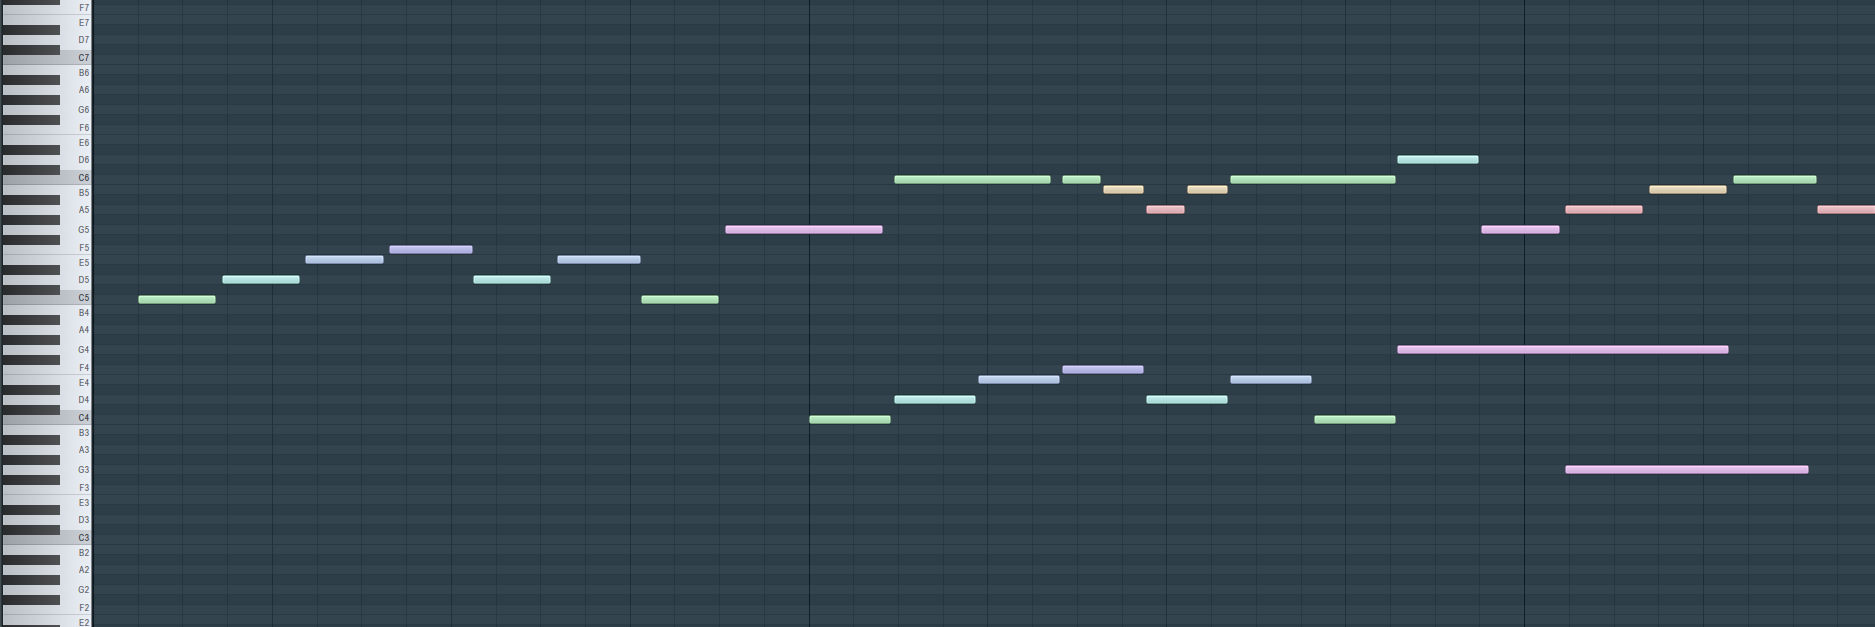
\includegraphics[width=.9\linewidth]{corpus-5.png}
  \captionof{figure}{First 30 Seconds - 'bwv772.mid'}
  \label{fig:test1}
\end{minipage}%
\begin{minipage}{.5\textwidth}
  \centering
  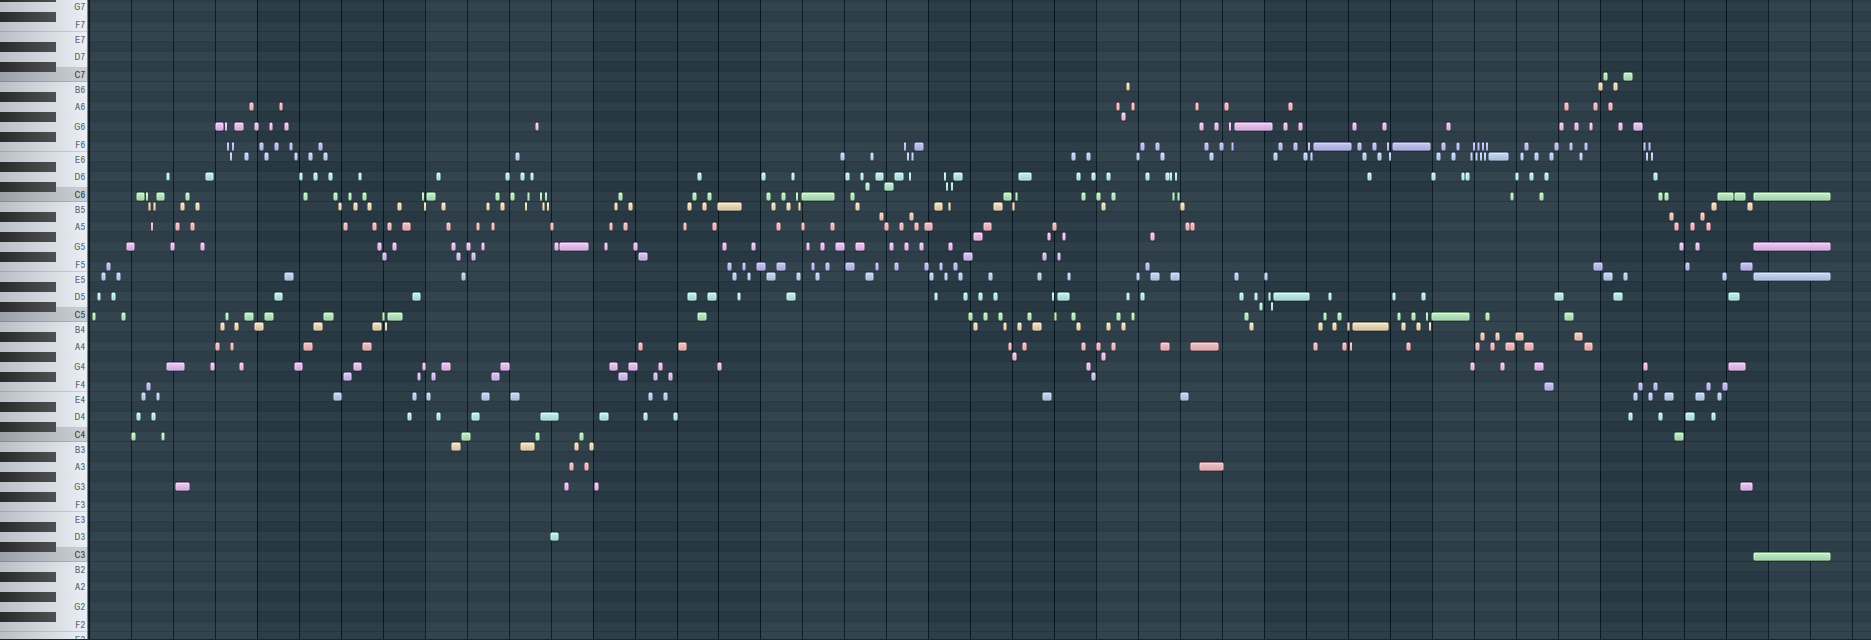
\includegraphics[width=.9\linewidth]{corpus-full.png}
  \captionof{figure}{Complete Piano Roll - 'bwv772.mid'}
  \label{fig:test2}
\end{minipage}

\centering
\begin{minipage}{.5\textwidth}
  \centering
  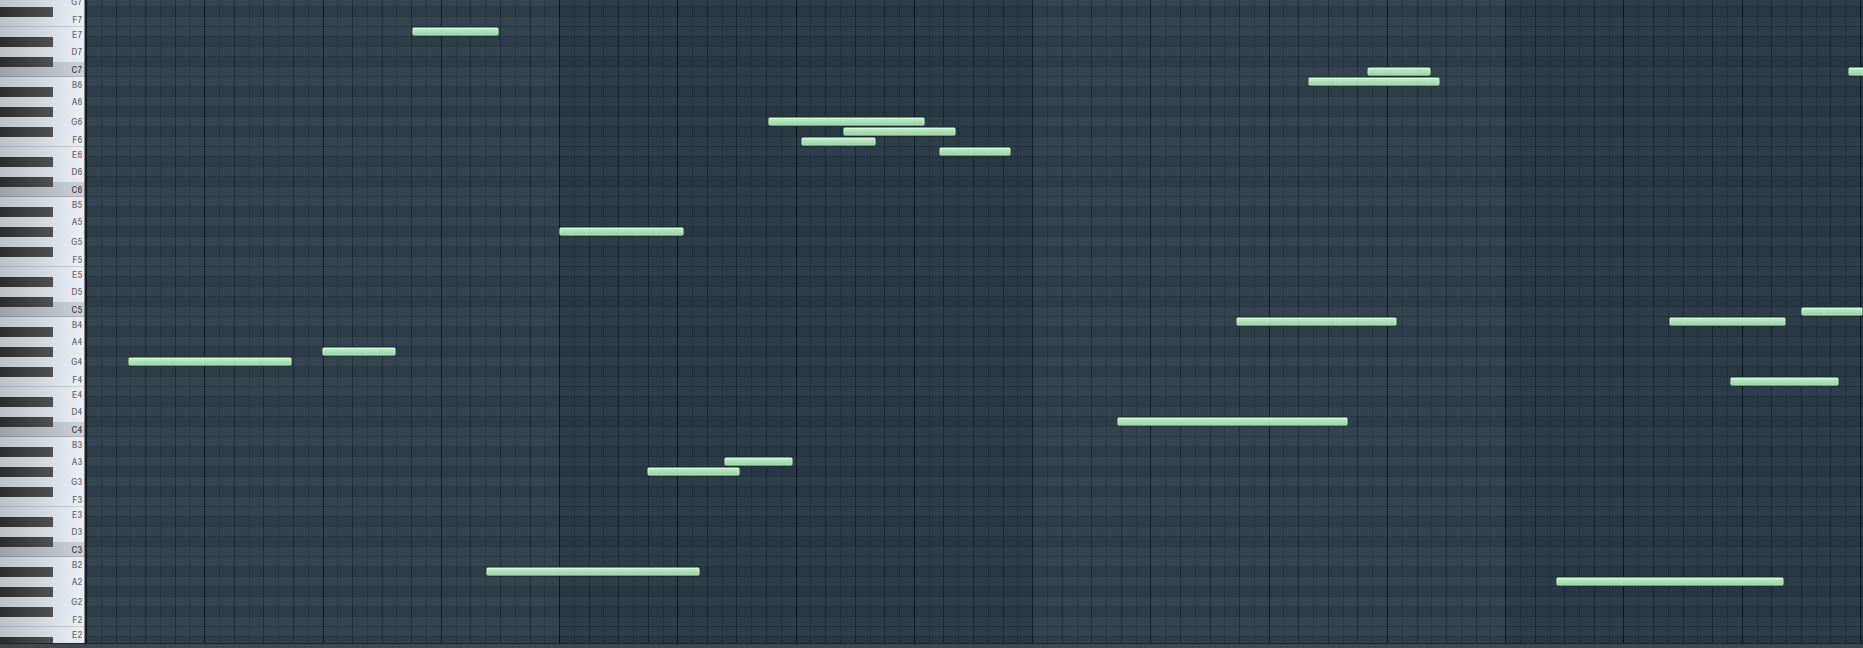
\includegraphics[width=.9\linewidth]{fitness1-first-30.png}
  \captionof{figure}{First 30 Seconds - Initial (Fitness 01)}
  \label{fig:test1}
\end{minipage}%
\begin{minipage}{.5\textwidth}
  \centering
  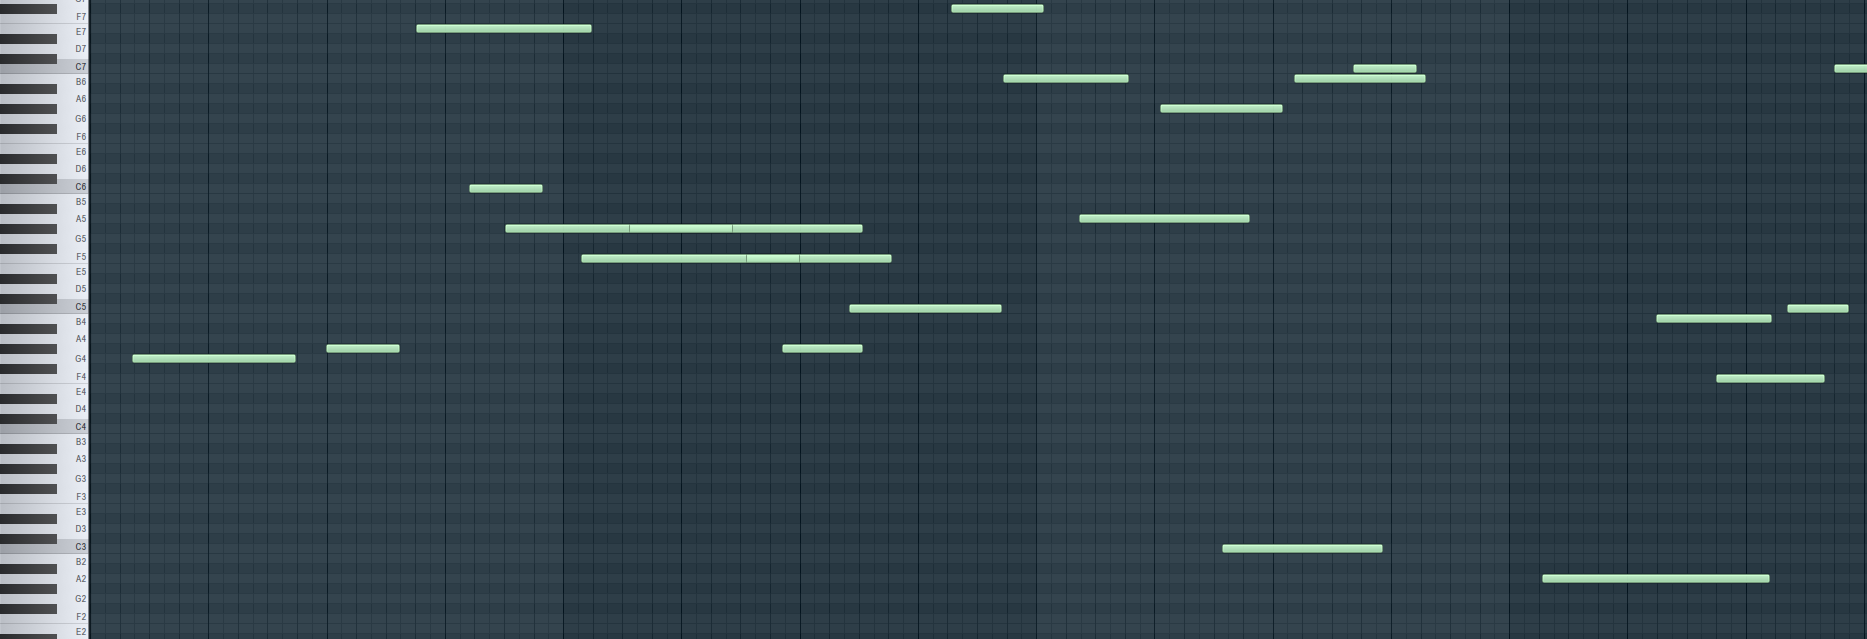
\includegraphics[width=.9\linewidth]{fitness1-final-30.png}
  \captionof{figure}{First 30 Seconds - Final (Fitness 01)}
  \label{fig:test2}
\end{minipage}

\centering
\begin{minipage}{.5\textwidth}
  \centering
  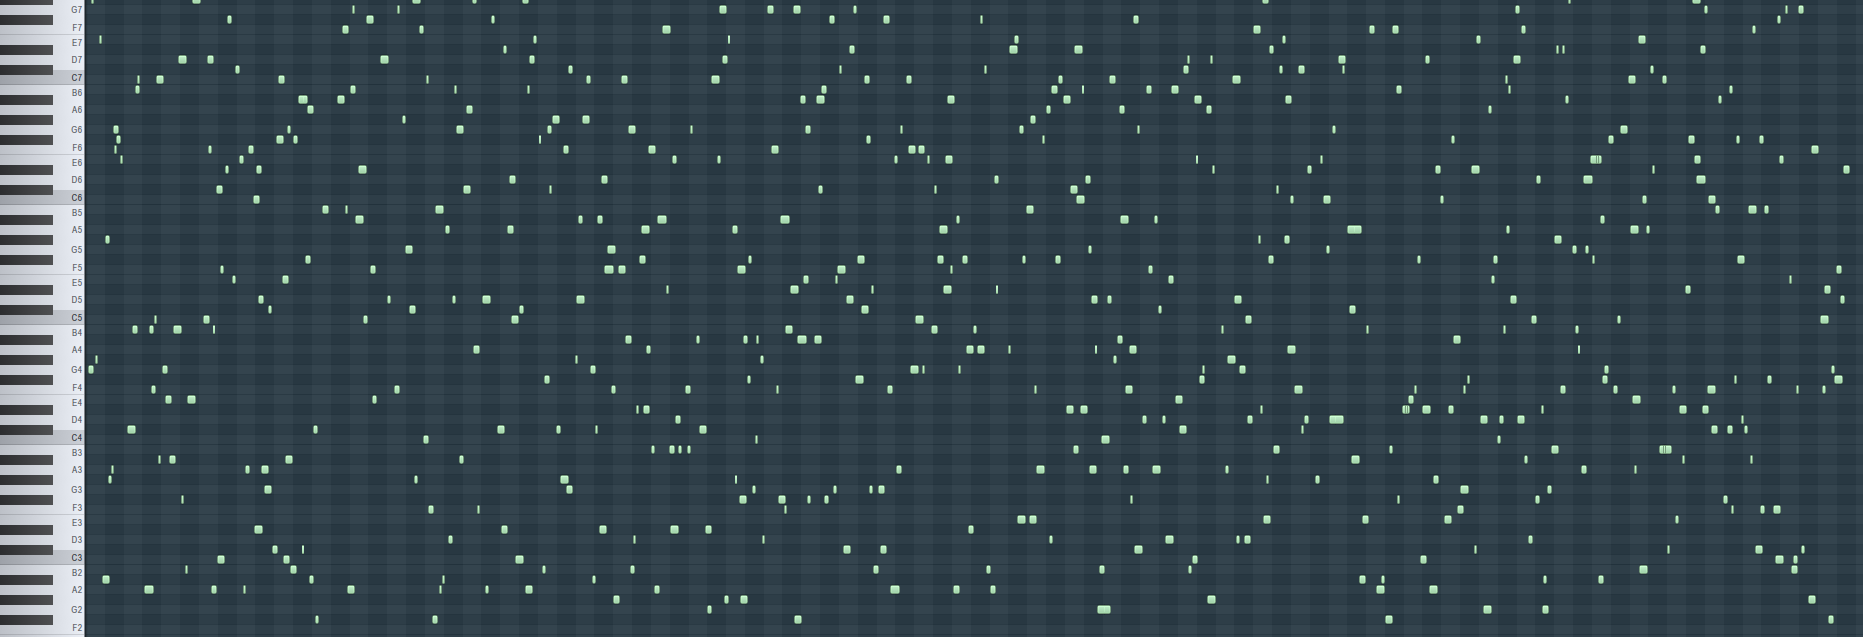
\includegraphics[width=.9\linewidth]{fitness1-first-full.png}
  \captionof{figure}{Complete Piano Roll - Initial (Fitness 01)}
  \label{fig:test1}
\end{minipage}%
\begin{minipage}{.5\textwidth}
  \centering
  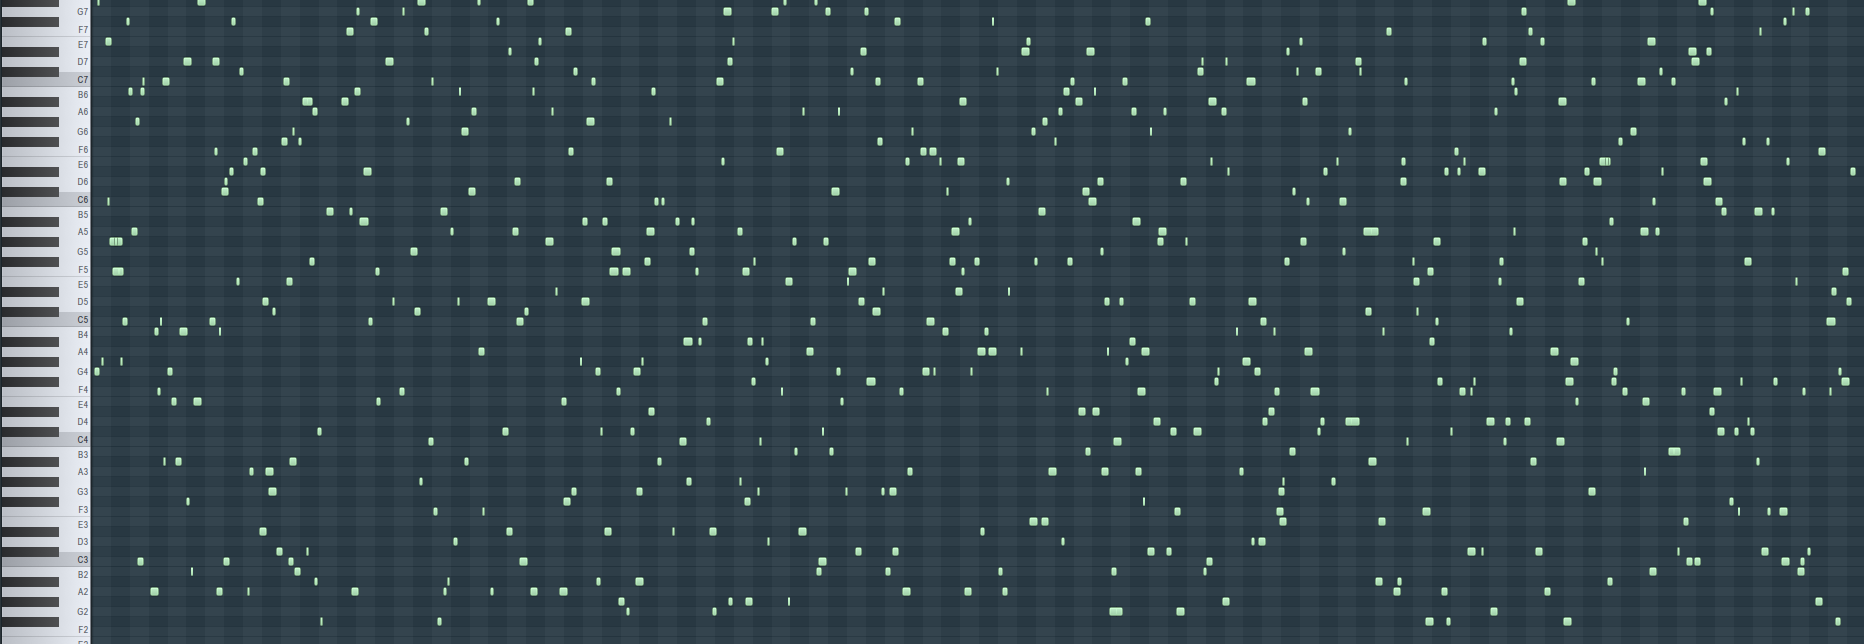
\includegraphics[width=.9\linewidth]{fitness1-final-full.png}
  \captionof{figure}{Complete Piano Roll - Final (Fitness 01)}
  \label{fig:test2}
\end{minipage}


\centering
\begin{minipage}{.5\textwidth}
  \centering
  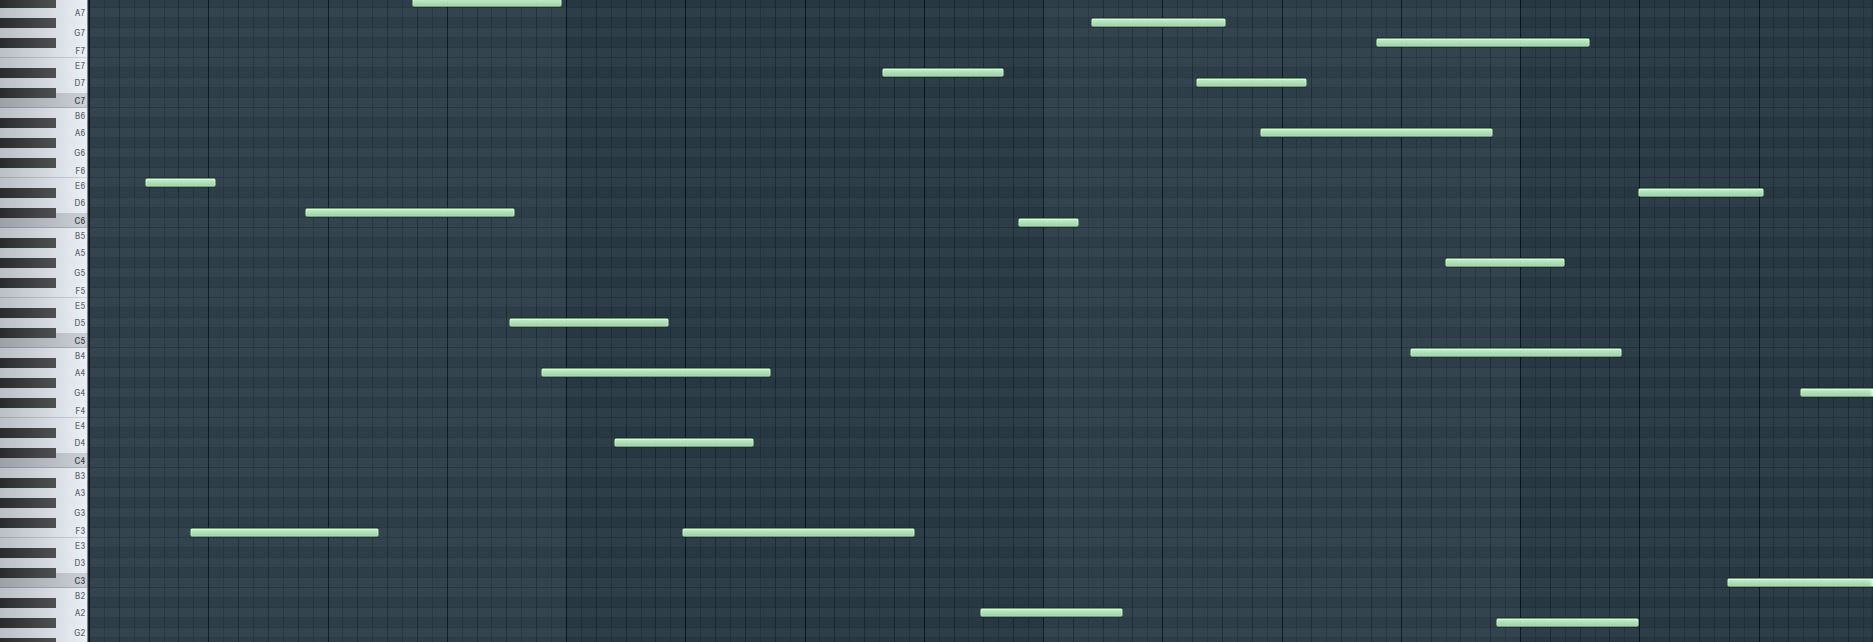
\includegraphics[width=.9\linewidth]{fitness2-first-30.png}
  \captionof{figure}{First 30 Seconds - Initial (Fitness 02)}
  \label{fig:test1}
\end{minipage}%
\begin{minipage}{.5\textwidth}
  \centering
  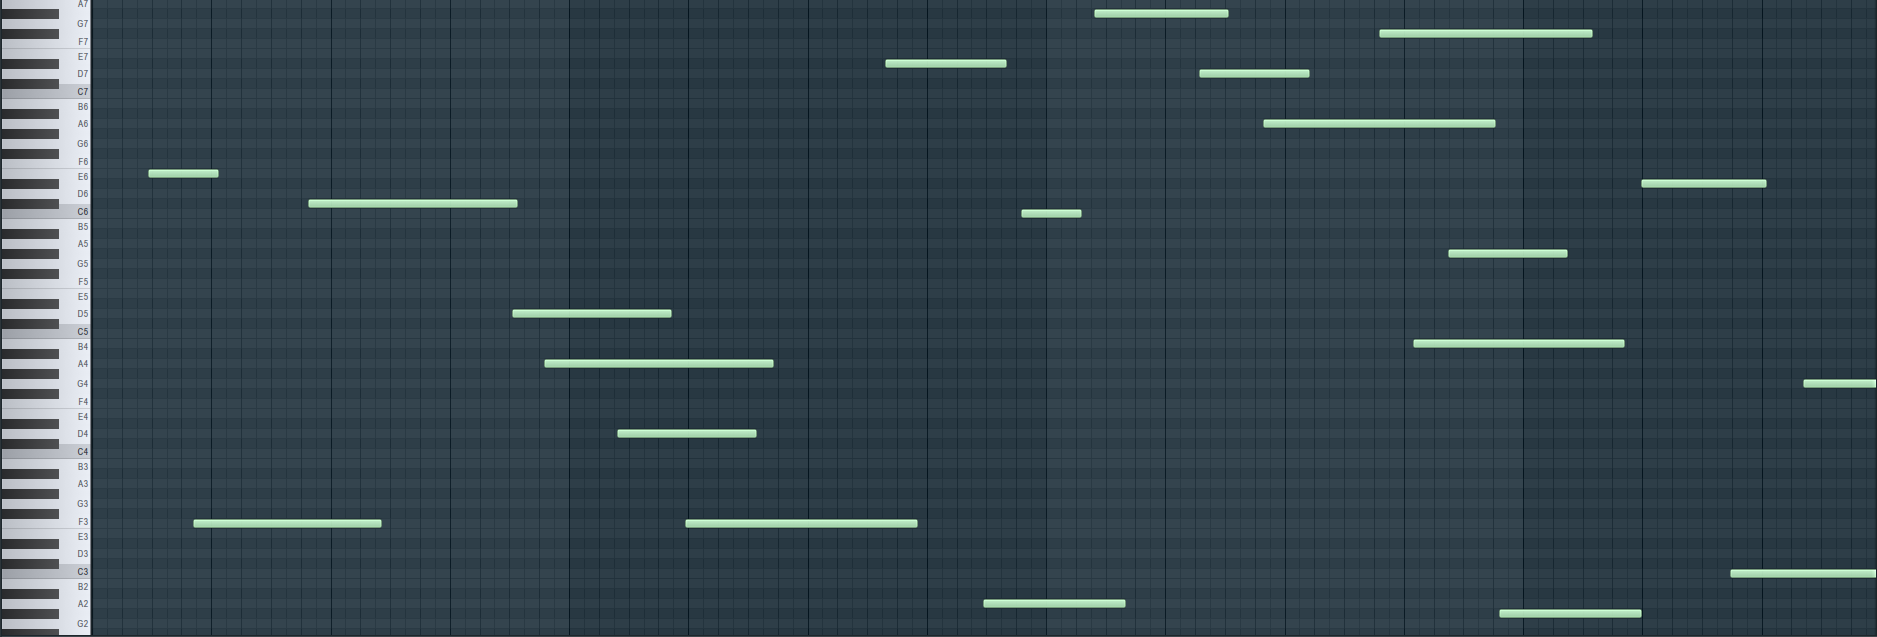
\includegraphics[width=.9\linewidth]{fitness2-final-30.png}
  \captionof{figure}{First 30 Seconds - Final (Fitness 02)}
  \label{fig:test2}
\end{minipage}

\centering
\begin{minipage}{.5\textwidth}
  \centering
  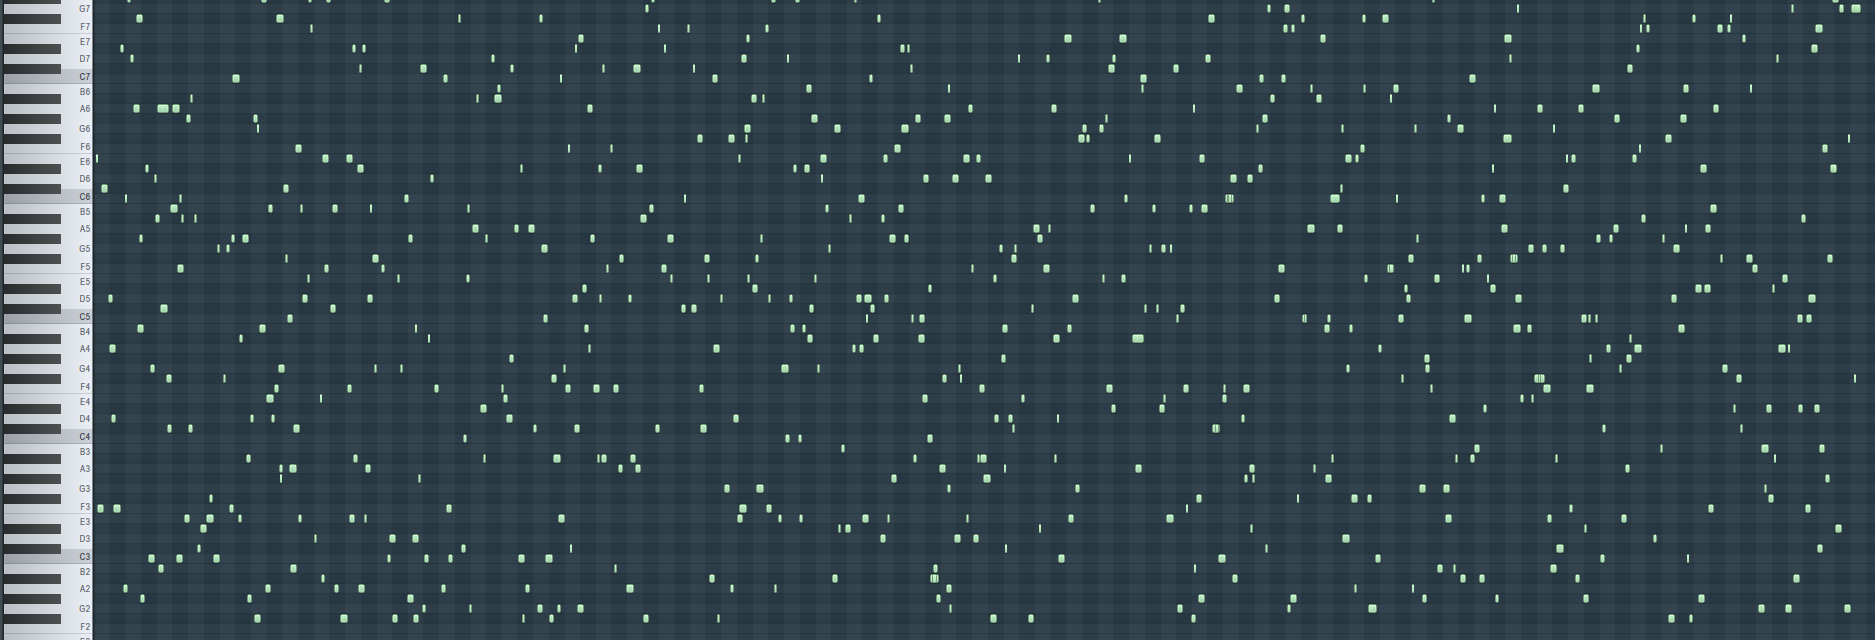
\includegraphics[width=.9\linewidth]{fitness2-first-full.png}
  \captionof{figure}{Complete Piano Roll - Initial (Fitness 02)}
  \label{fig:test1}
\end{minipage}%
\begin{minipage}{.5\textwidth}
  \centering
  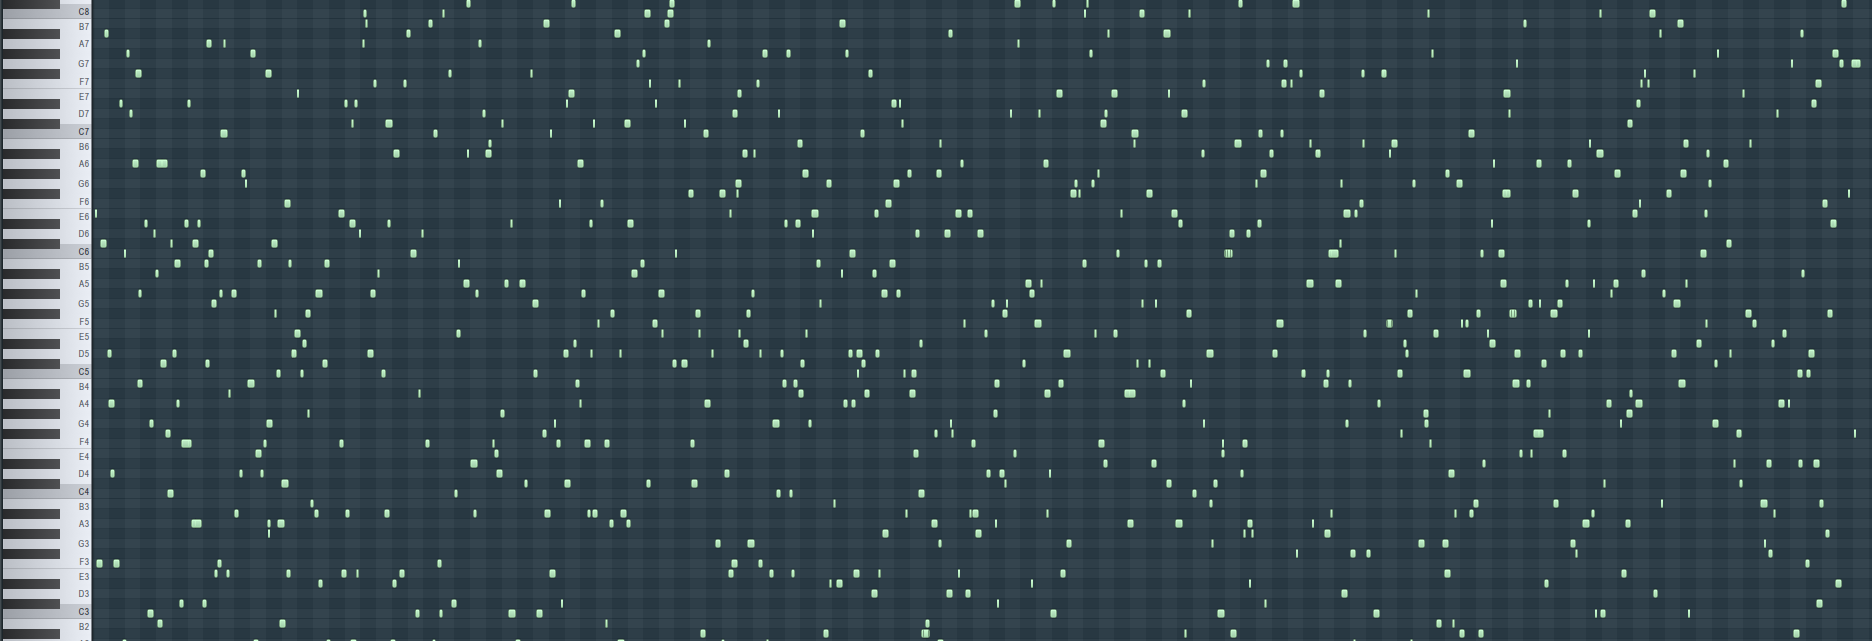
\includegraphics[width=.9\linewidth]{fitness2-final-full.png}
  \captionof{figure}{Complete Piano Roll - Final (Fitness 02)}
  \label{fig:test2}
\end{minipage}

\centering
\begin{minipage}{.5\textwidth}
  \centering
  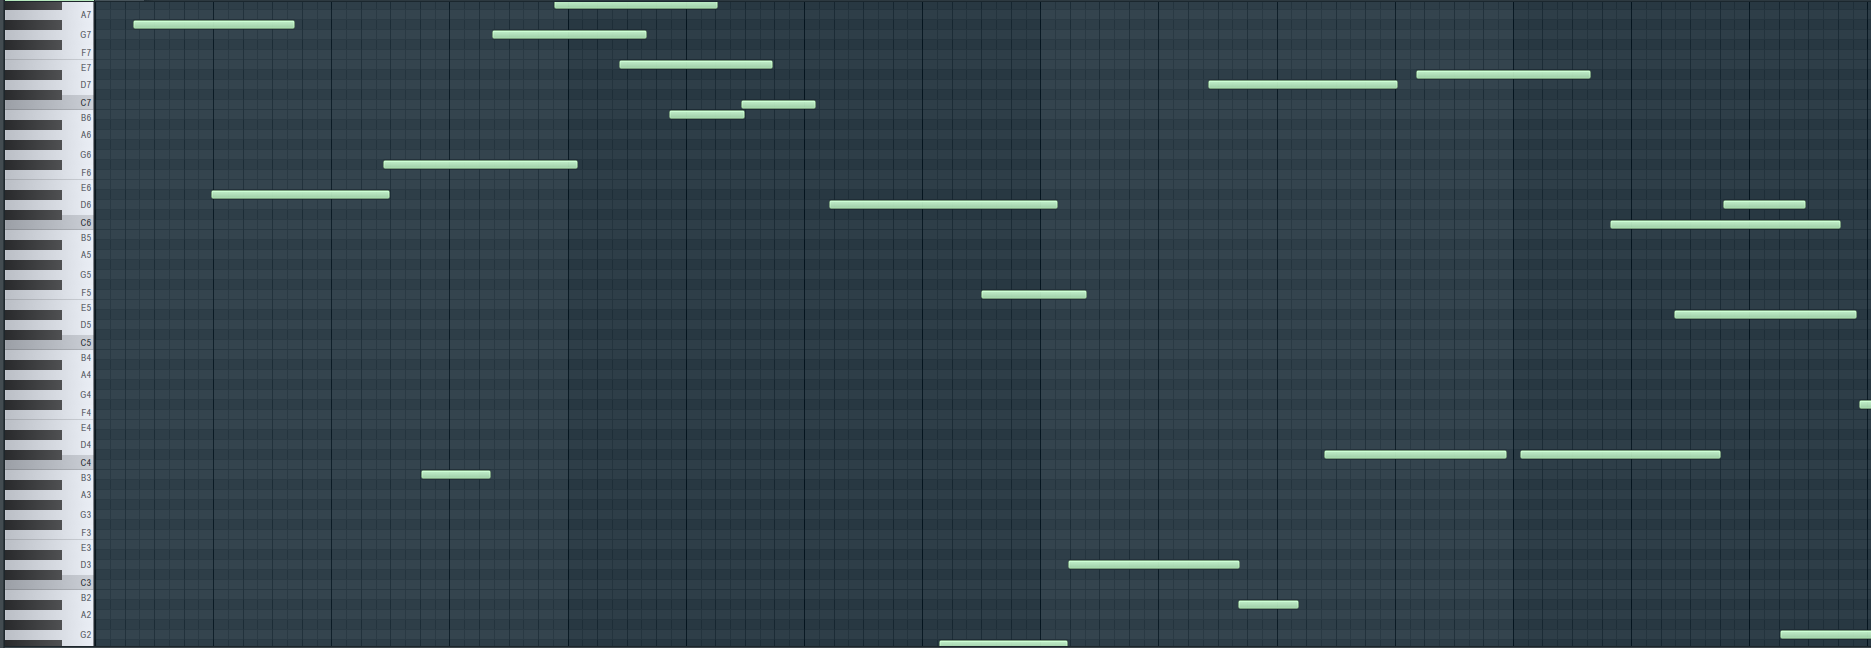
\includegraphics[width=.9\linewidth]{fitness3-first-30.png}
  \captionof{figure}{First 30 Seconds - Initial (Fitness 03)}
  \label{fig:test1}
\end{minipage}%
\begin{minipage}{.5\textwidth}
  \centering
  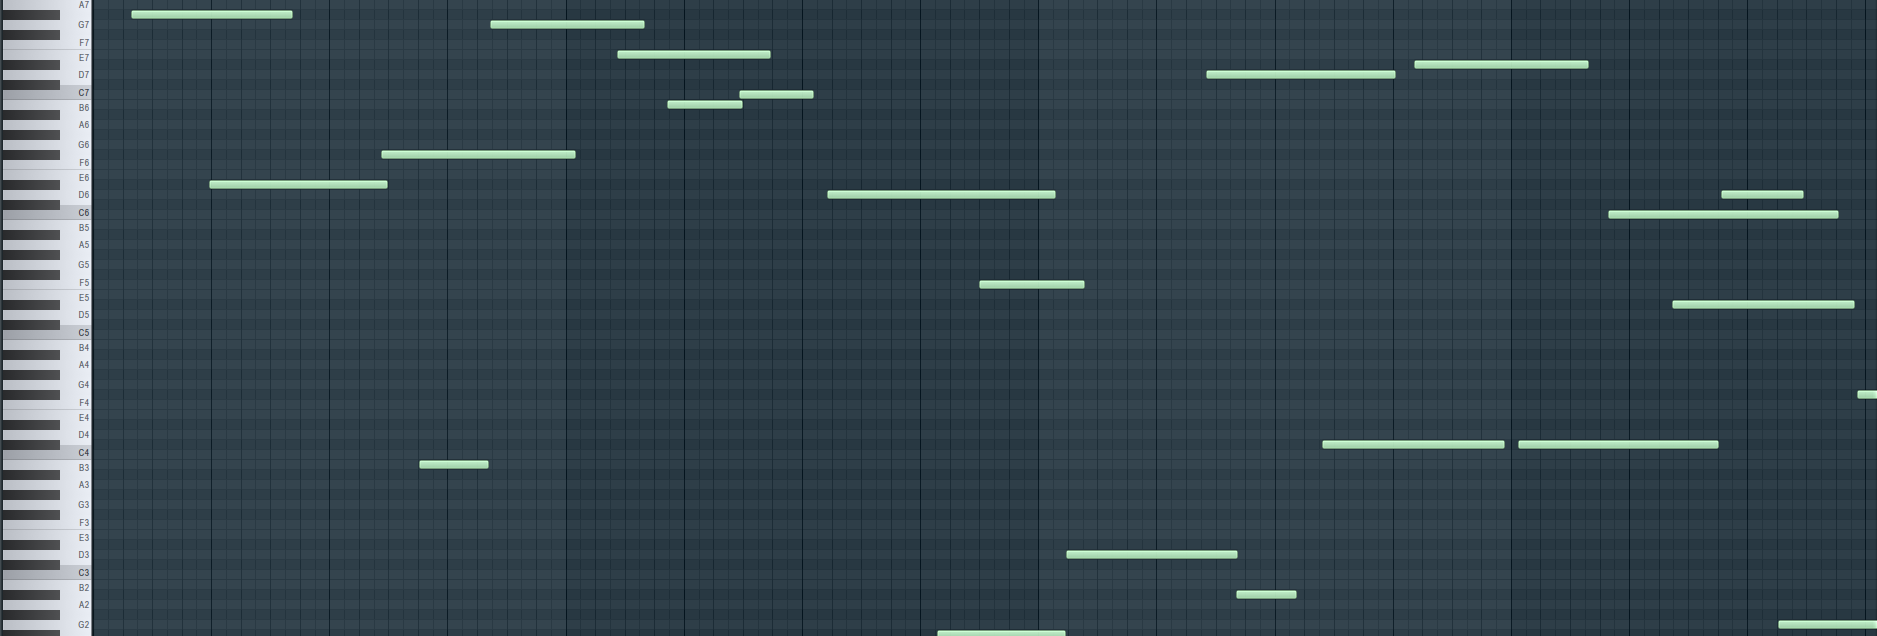
\includegraphics[width=.9\linewidth]{fitness3-final-30.png}
  \captionof{figure}{First 30 Seconds - Final (Fitness 03)}
  \label{fig:test2}
\end{minipage}

\centering
\begin{minipage}{.5\textwidth}
  \centering
  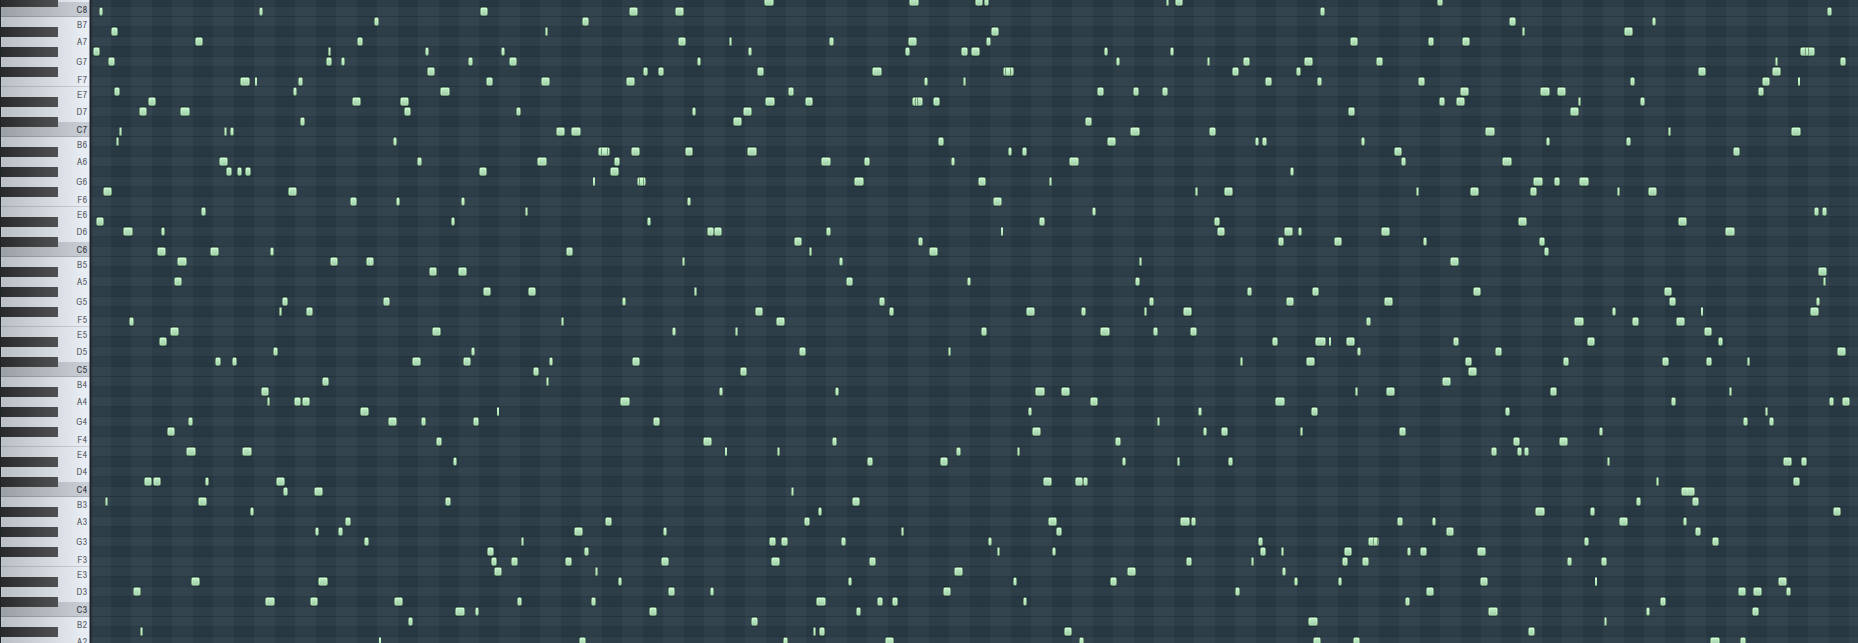
\includegraphics[width=.9\linewidth]{fitness3-first-full.png}
  \captionof{figure}{Complete Piano Roll - Initial (Fitness 03)}
  \label{fig:test1}
\end{minipage}%
\begin{minipage}{.5\textwidth}
  \centering
  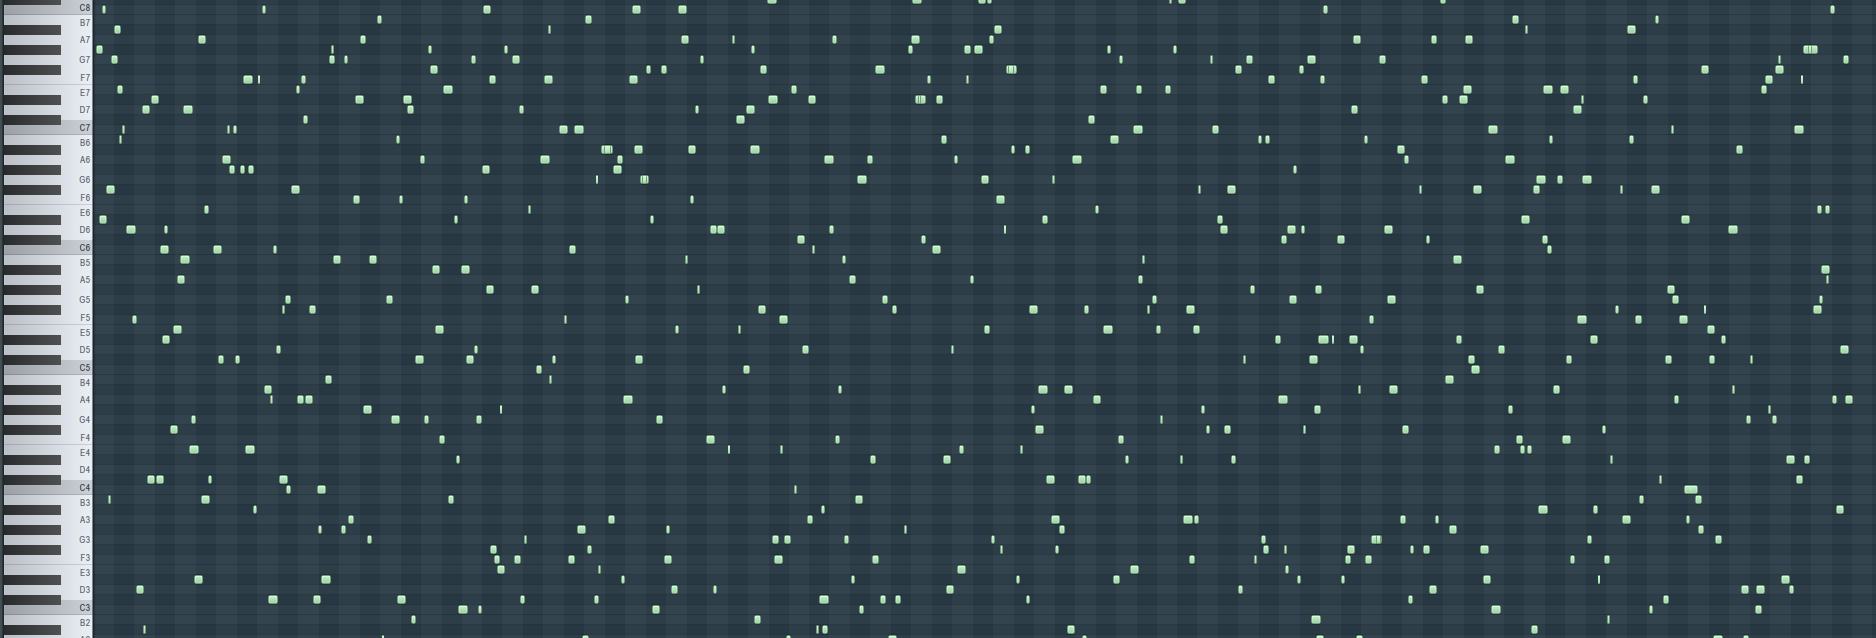
\includegraphics[width=.9\linewidth]{fitness3-final-full.png}
  \captionof{figure}{Complete Piano Roll - Final (Fitness 03)}
  \label{fig:test2}
\end{minipage}


\end{figure}

\end{document}
